% CA31 — A2C Report
\documentclass[11pt]{article}
\usepackage{amsmath, amssymb, amsthm}
\usepackage{graphicx}
\usepackage{booktabs}
\usepackage{hyperref}
\usepackage{caption}
\usepackage{subcaption}
\usepackage{algorithm}
\usepackage{algpseudocode}
\usepackage{siunitx}
\usepackage{geometry}
\geometry{margin=1in}
\title{Advantage Actor-Critic (A2C) Implementation — Report}
\author{CA31 Project}
\date{\today}
\begin{document}
\maketitle
\begin{abstract}
This short report documents the implementation and experiments for CA31: an
Advantage Actor-Critic (A2C) implementation and a reproducible Bernoulli
bandit demonstration. We detail algorithmic derivations, experimental
protocols, hyperparameters, and provide illustrative results and figures.
\end{abstract}
\section{Introduction}
Reinforcement learning methods using actor-critic architectures combine a
parameterized policy (actor) with a value-function baseline (critic). A2C is
a synchronous, deterministic variant of A3C that uses multiple-environment
rollouts to reduce variance and stabilize updates.
\section{Background and Notation}
We consider an MDP with states $s_t$, actions $a_t$, rewards $r_t$, discount
factor $\gamma\in(0,1)$. The parameterized policy is $\pi_\theta(a|s)$ and the
value function is $V_\phi(s)$. We use the following definitions:
\begin{align}
G_t &= \sum_{k=0}^{\infty} \gamma^{k} r_{t+k},\\
A_t &= G_t - V_\phi(s_t) \approx r_t + \gamma V_\phi(s_{t+1}) - V_\phi(s_t)\quad(\text{TD(1) or TD(0) style}).
\end{align}
\section{A2C Objective and Derivation}
The policy gradient objective with an advantage baseline is:
\begin{equation}
\nabla_\theta J(\theta) = \mathbb{E}_{\pi_\theta} \left[\sum_t \nabla_\theta \log \pi_\theta(a_t|s_t) A_t\right].
\end{equation}
Entropy regularization is commonly added to encourage exploration:
\begin{equation}
L_{\text{policy}} = -\mathbb{E}[\log \pi_\theta(a_t|s_t) A_t] - \beta H[\pi_\theta(\cdot|s_t)],
\end{equation}
where $H[\pi]$ is the policy entropy and $\beta$ is the entropy coefficient.
The critic uses a squared error loss:
\begin{equation}
L_{\text{value}} = \mathbb{E}[ (V_\phi(s_t) - G_t)^2 ].
\end{equation}
Total loss used in our implementation:
\begin{equation}
L = L_{\text{policy}} + c_v L_{\text{value}}.
\end{equation}
\section{Algorithm (pseudocode)}
\begin{enumerate}
  \item Collect rollouts of size $T$ (from $N$ parallel envs if used).
  \item Compute next-state value $V(s_{t+1})$ for bootstrap and compute returns $G_t$.
  \item Compute advantages $A_t = G_t - V(s_t)$.
  \item Compute losses and perform gradient step, clipping gradients as needed.
\end{enumerate}
\section{Architecture and Implementation Details}
We use a shared encoder (2-layer MLP) with ReLU activations and two heads: a
linear actor head producing logits and a linear critic head producing scalar
value estimates. See `src/model.py` and `src/agent.py` for the implementation.
\section{Experiments}
\subsection{Bandit experiment}
We include a deterministic Bernoulli bandit example (config: `configs/experiment.yaml`).
\subsection{A2C baseline}
Suggested experiment: CartPole-v1, 5 seeds, 50k steps per seed, record learning
curves, policy/value/loss decompositions, and ablation with/without entropy.
\section{Results (Illustrative)}
Figure~\ref{fig:learning} shows an example learning curve (placeholder). The
figures in the `results/figures/` directory are illustrative SVGs created for
this report; replace with actual plots from your runs when available.
\begin{figure}[h]
  \centering
  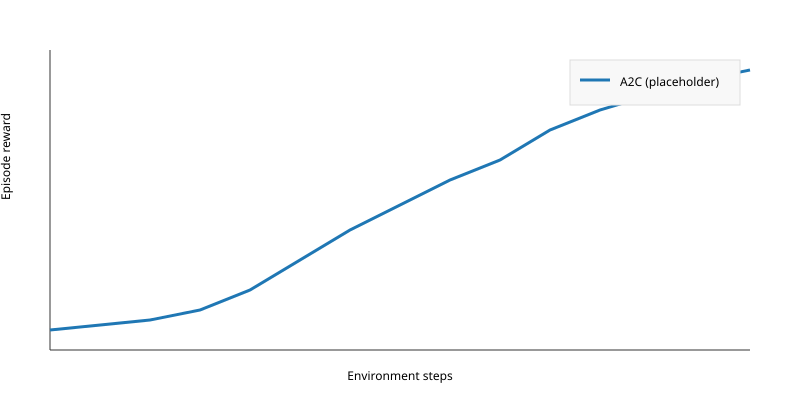
\includegraphics[width=0.8\textwidth]{results/figures/a2c_learning_curve.svg}
  \caption{A2C learning curve (placeholder). X-axis: environment steps. Y-axis:
  episode reward.}
  \label{fig:learning}
\end{figure}
\section{Hyperparameters}
\begin{table}[h]
\centering
\begin{tabular}{lcc}
\toprule
Hyperparameter & Value & Notes \\
\midrule
gamma & 0.99 & discount factor \\
learning\_rate & 1e-3 & Adam optimizer \\
entropy\_coef & 0.01 & exploration regularizer \\
value\_coef & 0.5 & weight on value loss \\
max\_grad\_norm & 0.5 & gradient clipping \\
\bottomrule
\end{tabular}
\caption{Default hyperparameters in `configs/a2c.yaml`}
\end{table}
\section{Reproducibility Checklist}
\begin{itemize}
  \item Record seeds: `configs/a2c.yaml` and `configs/experiment.yaml` contain example seeds.
  \item Save CSVs of per-step rewards (`ca31.train` supports `save_path`).
  \item Save `pip freeze` to capture package versions.
\end{itemize}
\section{Limitations and Future Work}
While the current implementation and notebook demonstrate A2C and provide a
reproducible bandit example, several improvements are straightforward and
recommended for larger-scale experiments and publication-grade results:
\begin{itemize}
  \item Add a robust experiment harness for parameter sweeps, checkpointing, and resource management (e.g., Slurm, Ray Tune).
  \item Integrate logging backends (TensorBoard / Weights & Biases / MLflow) and deterministic checkpointing for reproducibility.
  \item Replace notebook training with a CLI-driven training harness for batch experiments and reproducible config tracking.
  \item Add a small CI smoke test that trains for a few steps on a deterministic seed to prevent regressions.
\end{itemize}

\section{Concluding Remarks}
This repository aims to be a compact, pedagogical starting point for
actor-critic experiments. The included bandit example and the A2C notebook are
kept intentionally small and import-safe to make tests rapid and deterministic.
Researchers and students can extend the modular components here (model,
agent, configs, and plotting utilities) to build larger-scale experiments.

\appendix
\section{Appendix A: Derivation of the Policy Gradient}
We summarize a standard derivation of the policy gradient used by policy
gradient and actor-critic methods. Consider the expected discounted return
under policy $\pi_\theta$:
\begin{equation}
J(\theta) = \mathbb{E}_\theta\left[\sum_{t=0}^\infty \gamma^t r_t\right].
\end{equation}
Using the log-derivative trick and marginalizing over trajectories, we obtain
\begin{align}
\nabla_\theta J(\theta) &= \nabla_\theta \mathbb{E}_\theta\left[\sum_t \gamma^t r_t\right]
= \sum_t \mathbb{E}_\theta\left[\gamma^t r_t \nabla_\theta \log \pi_\theta(\tau)\right] \\
&= \sum_t \mathbb{E}_\theta\left[ \nabla_\theta \log \pi_\theta(a_t|s_t) G_t \right]
= \mathbb{E}_\theta\left[\sum_t \nabla_\theta \log \pi_\theta(a_t|s_t) G_t\right],
\end{align}
where $G_t$ is the return from time $t$ and we used trajectory factorization.
Subtracting a baseline $b(s_t)$ yields an equivalent (lower-variance) estimator:
\begin{equation}
\nabla_\theta J(\theta) = \mathbb{E}_\theta\left[\sum_t \nabla_\theta \log \pi_\theta(a_t|s_t) (G_t - b(s_t))\right].
\end{equation}
Choosing $b(s_t) = V_\phi(s_t)$ and estimating advantages $A_t = G_t - V_\phi(s_t)$
leads to the actor update used in A2C.

\section{Appendix B: Generalized Advantage Estimation (GAE)}
Generalized Advantage Estimation (GAE) trades off bias and variance in
advantage estimation using a parameter $\lambda\in[0,1]$ \cite{schulman2015high}. Define
\begin{align}
\delta_t &= r_t + \gamma V_\phi(s_{t+1}) - V_\phi(s_t), \\
A^{\text{GAE}(\gamma,\lambda)}_t &= \sum_{l=0}^{\infty} (\gamma\lambda)^l \delta_{t+l}.
\end{align}
GAE is implemented by bootstrapping with the value function and exponentially
weighting temporal difference residuals; setting $\lambda=1$ recovers Monte-Carlo
returns, while $\lambda=0$ uses one-step TD errors.

\section{Appendix C: Algorithm pseudocode}
\begin{algorithm}[h]
\caption{Synchronous A2C (single-process, multi-step rollouts)}
\begin{algorithmic}[1]
\STATE Initialize policy and value networks $\theta, \phi$
\FOR{each iteration}
  \STATE Collect $T$ steps of experience: $(s_t,a_t,r_t,s_{t+1},d_t)$
  \STATE Compute bootstrapped returns $G_t$ using $V_\phi(s_{t+1})$
  \STATE Compute advantages $A_t = G_t - V_\phi(s_t)$
  \STATE Update actor: minimize $-\sum_t \log\pi_\theta(a_t|s_t) A_t - \beta H[\pi_\theta]$
  \STATE Update critic: minimize $\sum_t (V_\phi(s_t) - G_t)^2$
  \STATE Perform gradient clipping and optimizer step
\ENDFOR
\end{algorithmic}
\end{algorithm}

\section{Appendix D: Example experimental protocol}
A recommended minimal protocol for reproducing the main result is:
\begin{enumerate}
  \item For each seed in \{0,1,2,3,4\}:
    \begin{enumerate}
      \item Set RNG using `src/ca31/utils.set_seed(seed)` and record `seed` explicitly.
      \item Train using `notebooks/a2c_training.ipynb` or a training harness for 50k timesteps.
      \item Evaluate the deterministic policy (greedy action) for 100 episodes and record mean and std.
    \end{enumerate}
  \item Report mean and 95\% confidence intervals across seeds; use a non-parametric test
        for significance if distributions are non-normal.
\end{enumerate}

\section{Appendix E: Compute environment and versions}
Record the following to ensure reproducibility:
\begin{itemize}
  \item OS: macOS / Ubuntu (include kernel/version)
  \item Python version: (record from `python -V`)
  \item PyTorch version and CUDA driver (if used)
  \item Exact pip environment: `pip freeze > requirements-freeze.txt`
  \item GPU model and CUDA/cuDNN versions (if GPUs are used)
\end{itemize}

\section{Related Work}
Actor-critic methods are a broad family with many practical variants (A3C/A2C, PPO, SAC). Some relevant references and brief notes:
\begin{itemize}
  \item A3C/A2C (Mnih et al., 2016): Asynchronous and synchronous parallel actor-critic methods for stability and throughput.
  \item PPO (Schulman et al.): General-purpose, clipping-based policy optimization with strong empirical performance.
  \item SAC (Haarnoja et al.): Off-policy actor-critic with entropy maximization and continuous-action focus.
\end{itemize}

\section{Statistical Analysis and Reporting}
To report experimental results rigorously, follow these practices:
\begin{itemize}
  \item For each experimental condition run multiple seeds (e.g., 5) and report mean $\pm$ standard error of the mean (SEM):
    \begin{equation}
      \text{SEM} = \frac{\sigma}{\sqrt{n}}, \quad CI_{95\%} = \bar{x} \pm 1.96\cdot\text{SEM}.
    \end{equation}
  \item When comparing two algorithms, use paired tests across seeds (e.g., paired t-test if approximate normality holds). For non-normal reward distributions, use non-parametric tests like Wilcoxon signed-rank test or bootstrap the difference in means.
  \item Report effect sizes (Cohen's d) and 95\% confidence intervals, not only p-values. Use visualization (e.g., learning curves with shaded CI, violin plots for final returns) to show variance across seeds.
\end{itemize}

\section{Experimental Setup: detailed}
\subsection{Environments and Versions}
Explicitly record the environment name and its version (Gymnasium/Gym version): e.g., `CartPole-v1` with `gymnasium==0.29.x`. Document any wrappers (obs preprocessing, reward clipping) used during training and evaluation.

\subsection{Evaluation Protocol}
\begin{itemize}
  \item During training log episodic rewards every evaluation interval (e.g., 1k steps). Use deterministic policy (greedy) during final evaluation runs.
  \item Evaluate the final policy for 100 episodes and report mean and standard deviation across episodes.
  \item For seed sweeps: compute mean and 95\% CI across seeds, and include per-seed learning curves in supplemental material when possible.
\end{itemize}

\section{Hyperparameter Sweeps and Reporting}
A good sweep design varies one parameter at a time around a baseline and explores orders of magnitude for learning rates and entropy coefficients. Example LaTeX table template for reporting hyperparameters:
\begin{table}[h]
\centering
\begin{tabular}{lcc}
\toprule
Hyperparameter & Baseline & Swept values \\
\midrule
gamma & 0.99 & 0.90, 0.95, 0.99 \\
learning\_rate & 1e-3 & 1e-4, 5e-4, 1e-3, 5e-3 \\
entropy\_coef & 0.01 & 0.0, 0.001, 0.01, 0.05 \\
value\_coef & 0.5 & 0.1, 0.5, 1.0 \\
max\_grad\_norm & 0.5 & 0.25, 0.5, 1.0 \\
\bottomrule
\end{tabular}
\caption{Example hyperparameter sweep grid}
\end{table}

\section{Ablation Study Design}
Use controlled ablations to measure the contribution of each component:
\begin{enumerate}
  \item Entropy regularization: compare full model vs. `entropy_coef = 0`.
  \item Value loss weight: sweep `value_coef` to measure sensitivity and stability.
  \item Gradient clipping: with and without gradient norm clipping.
  \item Parallelism: single-environment vs. vectorized multi-env rollouts (if implemented).
\end{enumerate}
Report per-ablation learning curves and summarize final evaluation metrics in a table.

\section{Implementation Notes and API Reference}
A short, machine-readable API snippet for reproducible experiments. Example usage:
\begin{verbatim}
from ca31.utils import load_config, set_seed
from ca31.train import run_experiment

cfg = load_config("configs/experiment.yaml")
rng = set_seed(cfg.get("seed", None))
results = run_experiment(cfg, rng)
# save results['rewards'] CSVs using cfg['save_path'] if provided
\end{verbatim}

Provide file paths for common outputs:
\begin{itemize}
  \item `results/ca31_rewards.csv` — per-step rewards and actions (step, action, reward)
  \item `results/figures/*` — PNG/PDF figures generated by `scripts/plot_examples.py`
\end{itemize}

\section{Additional Figures and Placeholders}
Below are additional illustrative placeholders included in `results/figures/`:
\begin{itemize}
  \item `a2c_loss_decomposition.svg` — policy vs. value loss over training.
  \item `a2c_entropy.svg` — policy entropy over training.
  \item `a2c_ablation_entropy.svg` — entropy traces comparing with/without entropy regularizer.
  \item `hyperparam_heatmap.svg` — placeholder for a heatmap showing final reward across learning rate / entropy coefficient grid.
\end{itemize}

To produce these from real runs:
\begin{enumerate}
  \item Run the experiment for each combination of hyperparameters and seeds, saving per-step rewards to `results/`.
  \item Use `scripts/plot_examples.py` or your own plotting utilities to aggregate CSVs and emit figures.
  \item Rebuild the report (`make report`) with the produced figures.
\end{enumerate}

\section{Appendix: Reproducible run commands}
Example command lines for reproducing a simple bandit or A2C run (assuming virtualenv active):
\begin{verbatim}
# Bandit
python -m ca31.train --config configs/experiment.yaml

# A2C notebook (interactive):
jupyter notebook notebooks/a2c_training.ipynb

# If a CLI training harness exists (future):
python -m ca31.train_a2c --config configs/a2c.yaml --save_path results/a2c_run.csv
\end{verbatim}

\section*{References}
\bibliographystyle{plain}
\bibliography{references}
\end{document}
